%% SECTION HEADER /////////////////////////////////////////////////////////////////////////////////////
\section{Sample Configuration}
\label{sec:sample}

%% SECTION CONTENT ////////////////////////////////////////////////////////////////////////////////////
The sample of interest was a \(500\times500\times1.5\) mm\(^3\) unidirectional \ac{cfrp} in stack sequence \([0^{\circ},90^{\circ}]_s\) plate bonded to an aluminium honeycomb core. 
It was decided to use only one skin, as it is pictured in Fig.~\ref{fig:honeycomb}(b), with the intention of experimental validation and to be able to enlarge disbonds between the skin and the core located in the middle of the \ac{hsc} with a tool in a real sample. 
It was not decided to dedicate separate samples for each size of damage because too many factors would affect the signal value, including skin and sensors properties, the thickness of the adhesive layers, position of the core relative to the sensors, and distance between sensor.
\begin{figure}[H]
	\begin{center}
		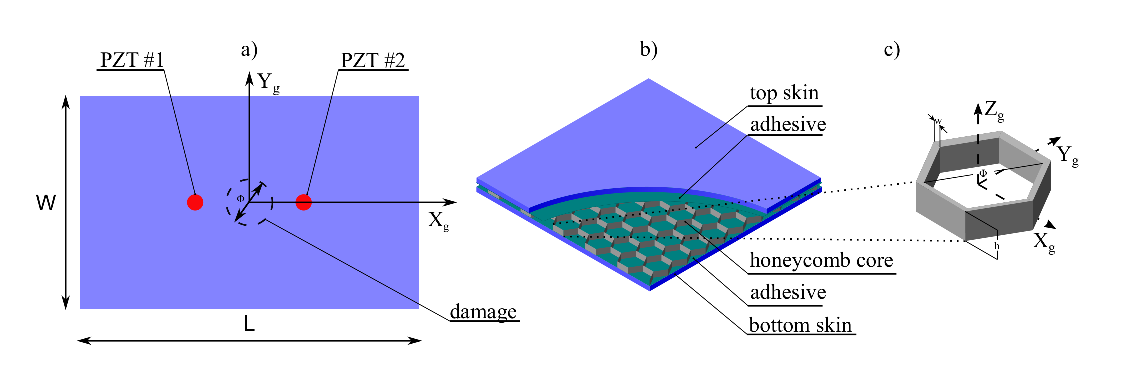
\includegraphics{Chapter_5/honeycomb}
	\end{center}
	\caption{Sample configuration: (\textbf{a}) top view of the sample, (\textbf{b}) honeycomb sandwich substructures and (\textbf{c}) details of the honeycomb cell.}
	\label{fig:honeycomb}
\end{figure}

The core geometry is accurately reproduced from the actual specimen, i.e., incorrect hexagonal \(\left(\mathrm{h}_1 \ne \mathrm{l}_1\right)\) and double walls at the sheet joints, resulting from the core fabrication technology.
According to the drawing in Fig.~\ref{fig:honeycomb}(\textbf{c}), the cell dimensions are w=0.1 mm, h\(_1\)=11 mm, h\(_2\)=5 mm, l\(_1\)=10.4 mm, l\(_2\)=6 mm and the cell height g=14.5 mm.
The core was bonded to one \ac{cfrp} plate using the epoxy adhesive (Loctite EA3479B) with the thickness h\(_a\)=0.3 mm.
The adhesive layer covered the entire bottom surface of the skin.

Signal excitation and recording were accomplished with a pair of \acp{pzt}  (Noliac, NCE51)mounted to the top surface of the skin with cyanoacrylate glue.
The circular transducers of diameter \(\Phi_{PZT}\)=10 mm and thickness h\(_{PZT}\)=0.5 mm were attached 200 mm apart, as shown in Fig.~\ref{fig:honeycomb}(\textbf{a}). The thickness of cyanoacrylate glue under \ac{pzt} was assumed to be h\(_g=50\) \(\mu\)m.

The material properties of the components needed for the simulations are compiled in Tab.~\ref{tab:properties}.
\begin{table}[H]
	\small
	\tabcolsep=0.75cm
	%	\centering
	\caption{\label{tab:properties}The mechanical properties of the materials.}
	\begin{tabular}{ccccc}\toprule
		\multirow{2}{*}{\textbf{Material}} & $\boldsymbol{E_{11}}$ & $\boldsymbol{E_{33}}$ & $\boldsymbol{\nu_{12}}$ & $\boldsymbol{\rho}$ \\ & GPa & GPa & -- & kg/m\(^3\)\\
		\midrule
		Carbon & 275 & 27 & 0.2 & 1900\\
		Epoxy & 3.43 & 3.43 & 0.35 & 1250\\
		Aluminium & 71 & 71 & 0.33 & 2770\\
		Epoxy adhesive & 6 & 6 & 0.34 & 1200\\
		Cyanoacrylate glue & 3 & 3 & 0.34 & 1200\\		
		\bottomrule
	\end{tabular}
\end{table}
